\documentclass[twocolumn,superscriptaddress]{revtex4-1}
\usepackage{color}
\usepackage{graphicx}
\usepackage{epstopdf}
\epstopdfsetup{update}
\usepackage{amsmath}
\usepackage{mathtools}
\usepackage[colorlinks,linkcolor=blue,anchorcolor=blue,citecolor=blue,urlcolor=blue]{hyperref}

%===============================================
\begin{document}
\title{Signatures of Deconfined Quantum Criticality in Half-Filled SU(6) Hubbard Model on a Square Lattice}
\author{Da Wang} \email{dawang@nju.edu.cn}
\affiliation{National Laboratory of Solid State Microstructures and School of Physics, Nanjing University, Nanjing 210093, China}
\author{Lei Wang} \email{wanglei@iphy.ac.cn}
\affiliation{Beijing National Lab for Condensed Matter Physics and Institute of Physics, Chinese Academy of Sciences, Beijing 100190, China}
\author{Congjun Wu} \email{cjwu@physics.ucsd.edu}
\affiliation{Department of Physics, University of California, San Diego, California 92093, USA}
\begin{abstract}
  The quantum phase transition between antiferromagnetism (AF) and valence bond solid (VBS) can be continuous due to the deconfined spinons at the quantum critical point (QCP). In this work, we report our numerical evidence of the continuous AF-VBS phase transition in half-filled SU(6) fermionic Hubbard model on a square lattice through quantum Monte Carlo simulations. The QCP $U_c=13.3(2)$ is determined by finite size scalings of structure factors and AF correlation lengths. Moreover, smooth energy evolution and emergent U(1) symmetry are observed strongly supporting the deconfined QCP as well. The anomalous dimensions $\eta_{\rm AF}=0.44(3)$ and $\eta_{\rm VBS}=0.98(2)$ are much larger than the SU(2) case and also differ from the fundamental representation described by the non compact CP$^{5}$ model. Here, the QCP belongs to the self-conjugate representation of the SU(6) spin and should be governed by a $U(6)/[U(3)\otimes U(3)]$ nonlinear sigma model calling for more elaborated theoretical investigations. 
\end{abstract}
\maketitle

\section{introduction}
Topological excitations play important roles in modern physics, especially in low dimensions. The deconfinement of vortices in two dimensional XY-model causes the Berezinskii-Kosterlitz-Thouless phase transition. \cite{Kosterlitz1973} While in 2+1 dimensional antiferromagnetic (AF) Heisenberg model, the topological excitations dubbed as hedgehogs can become deconfined and lead the AF phase to a paramagnetic phase by their condensation. \cite{Haldane1988a} Such a magnetic disordering phase can also break lattice symmetry, known as spin-Peierls or valence-bond-solid (VBS) state. \cite{Read1989b,*Read1989a,*Read1990} According to Landau-Ginzburg-Wilson theory, the AF-VBS phase transition should be of first order because they break different symmetries. But from the viewpoint of topological excitations, i.e. hedgehogs in AF and vortices in VBS, the AF-VBS transition is proposed to be a continuous one named as deconfined quantum criticality due to the deconfined topological excitations at the quantum critical point (QCP). \cite{Senthil2004,*Senthil2004a,*Levin2004} The deconfined QCP was first proposed on a non-compact CP$^1$ model and later received much attention in recent years. By many efforts, it has been confirmed numerically on some designer models such as J-Q \cite{Sandvik2007,Melko2008,Sandvik2010,Pujari2013,Shao2016}, classical loop \cite{Nahum2015}, J$_1$-J$_2$ \cite{Wang2016d} and gauged fermionic \cite{Assaad2016} models. But there are also some other models \cite{Kragset2006,Kuklov2006,Sen2010,Papanikolaou2010} (even including the non compact CP$^1$ model itself\cite{Kuklov2008}) which are found to be of first order and thus may not be deconfined QCPs. 

The studies have also been extended to higher symmetries, e.g. SO(N)\cite{Kaul2015} and SU(N)
groups\cite{Lou2009,Kaul2012a,Kaul2012,Block2013,D'Emidio2016,D'Emidio2017}. One motivation is the large-N limit can be solved perturbatively. \cite{Affleck1988a,Marston1989,Arovas1988,Read1989b,*Read1989a,*Read1990,Auerbach2011} Another motivation is that: higher symmetry always brings us more surprises and can unify different phenomena in the sense of low energy effective theories \cite{Hooft2005,Zhang1997,Volovik2003,Hayward2014,Nahum2015a}, or even in bare models directly like in cold atom experiments. \cite{Wu2003,*Wu2006a,DeSalvo2010,Taie2010,Krauser2012,Taie2012,Zhang2014,Cazalilla2014,Laflamme2016} 


%\begin{figure}
%  \begin{flushleft}
%    \includegraphics[width=0.42\textwidth]{su63.jpg}
%    \includegraphics[width=0.30\textwidth]{su61.jpg}
%    \caption{\label{fig:su6}Sketch of SU(6) AF and VBS. (a) and (b) give AF and VBS configurations within the self-conjugate representation which is studied in this work. There are three fermions at each site with flavors represented by six colors.  As a comparison, we also show the fundamental representation in (c) and (d) in which there are one and five fermions at two sublattices, respectively. }
%  \end{flushleft}
%\end{figure}
%

When talking about SU(N) AF and VBS, we need first to specify their meanings. Mathematically, an SU(N) spin can be
represented by a Young tableau with $p$ rows and $n_c$ columns of boxes, each of which can be filled with one of N
values. \cite{Affleck1985,Read1989b,*Read1989a,*Read1990} The extensively studied case in literature
\cite{Harada2003,Kawashima2007,Lou2009,Kaul2012a,Kaul2012,Block2013,D'Emidio2016,D'Emidio2017} is called fundamental representation with $n_c=p=1$, in which case there is only one particle in A site and $N-1$ particles in B site. The two sites can form a large singlet in the VBS state or keeps frozen to be opposite in the AF state. In large $n_c$ limit, such a representation is a direct generalization of the CP$^{1}$ model, called CP$^{N-1}$ model. \cite{Halperin1974,Read1989b,*Read1989a,*Read1990}
In this work, we focus on another type of AF and VBS, called self-conjugate representation with $n_c=1$ and $p=N/2$. In this ground state, there are both N/2 particles in A and B sites. 
%The two sites can form a large singlet by switching one, two and three pairs of particles. 
To the best of our knowledge, detailed properties of such a AF-VBS transition has received few attentions in literature. \cite{Wang2014b,Lang2015}. By symmetry analysis, from the AF side, the phase transition is known to be described by a $ U(N)/[U(N/2)\otimes U(N/2)]$ nonlinear sigma model \cite{MacFarlane1979,Duerksen1981,Read1989b,*Read1989a,*Read1990} different from the CP$^{N-1}$ model. As a result, it must belong to a new universality class, if the AF-VBS phase transition is really a continuous one. 
%At first sight, let us examine the topological excitations of the self-conjugate VBS state, as plotted in Fig.~\ref{fig:spinon} taking SU(6) case as an example. The vortex is constructed by three fermions (or spinons when charge fluctuations are suppressed), regardless of the VBS types (columnar or plaquette). This is fundamentally different from the CP$^{N-1}$ theory, where the vertex has no internal structure. On the other hand, from the AF side, the phase transition is well known to be described by a non-linear sigma model on a $ U(N)/[U(N/2)\otimes U(N/2)]$ Grassman manifold, \cite{MacFarlane1979,Duerksen1981,Read1989b,*Read1989a,*Read1990} again different from the CP$^{N-1}$ theory. As a result, it is reasonable to expect a new universality class in the self-conjugate representation, if the AF-VBS phase transition is a continuous one. 


In fact, the self-conjugate represented AF/VBS can readily exist in the half-filled SU(N) Hubbard model, \cite{Honerkamp2004,Assaad2005,Cai2013a,Cai2013,Wang2014b,Zhou2014} \footnote{The SU(N) Hubbard model can also host the fundamental (or generally $p$-rows) represented AF/VBS by choosing different onsite energies on two sublattices to obtain different particle numbers. But this will cause sign problem in determinant QMC and thus prevent large scale calculations.} which has already been realized in cold atom experiments. \cite{Taie2012,Zhang2014,Cazalilla2014} Our previous study\cite{Wang2014b} of this model on a square lattice has identified the existence of AF for small Hubbard $U$ in both SU(4) and SU(6) cases due to Fermi surface nesting and divergence of normal state density of states. However, different from the SU(2) case where the AF moment saturates as $U$ increases, the SU(4) and SU(6) AF moments shows non-monotonic behaviors. For the SU(6) model, AF is eventually killed and substituted by a VBS order. Investigating the critical property of this AF-VBS phase transition is the main task of this work. Through large scale projecting determinant quantum Monte Carlo (QMC) simulations, we have found indications of the deconfined quantum criticality for the self-conjugate represented SU(6) AF-VBS transition. Moreover, the critical exponents indicate the QCP belongs to a new universality class beyond the fundamental represented SU(N) or equivalently non compact CP$^{N-1}$ theory.

%\begin{figure}
%  \includegraphics[width=0.5\textwidth]{spinon}
%  \caption{\label{fig:spinon}Vortex of Z4 VBS. For both columnar and plaquette VBSs, the vortex is a three-fermion state. In low energy theory with charge excitation forbidden, the vortex is constructed by three spinons. Therefore, there are $C_6^3=20$ kinds of vortices altogether.}
%\end{figure}


\section{model and QMC simulations}
The SU(N) Hubbard model is written as
\begin{eqnarray}
  H=-t\sum_{\langle i,j\rangle,\alpha}\left(c_{i\alpha}^\dag c_{j\alpha}
  +h.c.\right)+\frac{U}{2}\sum_{i}\left(n_i-\frac{N}{2}\right)^2
  \label{eq:hamilton}
\end{eqnarray}
where $c_{i\alpha}$ is a fermionic annihilation operator with $i$ a site index and $\alpha$ a flavor index satisfying $1\le\alpha\le N$. The first term represents hoppings between nearest neighbour sites with hopping integral $t$ which is set as $1$ throughout this work. The second term describes onsite Coulomb interactions with Hubbard $U$ and $n_i=\sum_{\alpha=1}^{N} c_{i\alpha}^\dag c_{i\alpha}$. 

On a bipartite lattice, the half-filling SU(N) (with even N) Hubbard model keeps invariant under a partial particle-hole transformation: $c_{i,\alpha>N/2}\rightarrow(-1)^i c_{i,\alpha>N/2}^\dag$. Such a transformation guarantees the model free of sign problem in determinant QMC simulations. \cite{Wu2005a} This enables us to perform large-scale projector QMC simulations to study this problem, particularly with $N=6$. Details of the algorithm can be found elsewhere. \cite{Assaad2008,Wang2014b,Zhou2016} In our simulations, projection time $\beta=2L$ is used, which is long enough to achieve convergence for a given $L$. The discrete time slice $\Delta\tau$ is chosen to be $0.05$. For each group of parameters, the simulation is performed on 24 cores (48 for $L=24$) with 1000 (500 for $L=24$) Monte Carlo steps to warm up and no less than 1000 (500 for $L=24$) steps for measurement on each core. 



\section{QMC results}

%\subsection{structure factors}



For the SU(6) Hubbard model, we are interested in the magnetic moment 
\begin{eqnarray}
  m_r=\frac{1}{6}\left( \sum_{\alpha=1}^{3}n_{r\alpha} -\sum_{\alpha=4}^{6}n_{r\alpha} \right)
\end{eqnarray}
with the largest value $1/2$ the same as SU(2) case. The AF moment is the Fourier transformation at momentum $(\pi,\pi)$, i.e. $m=\frac{1}{L^2}\sum_{r}m_r(-1)^r$ where momentum is omitted for simplicity unless otherwise specified. In finite size QMC simulations, symmetry is not broken so that we instead measure the AF structure factor (equal-time correlation) directly
\begin{eqnarray}
  \langle m^2 \rangle=\frac{1}{L^4}\sum_{rr'}\langle m_rm_{r'}\rangle (-1)^{r-r'}
\end{eqnarray}

\begin{figure}
	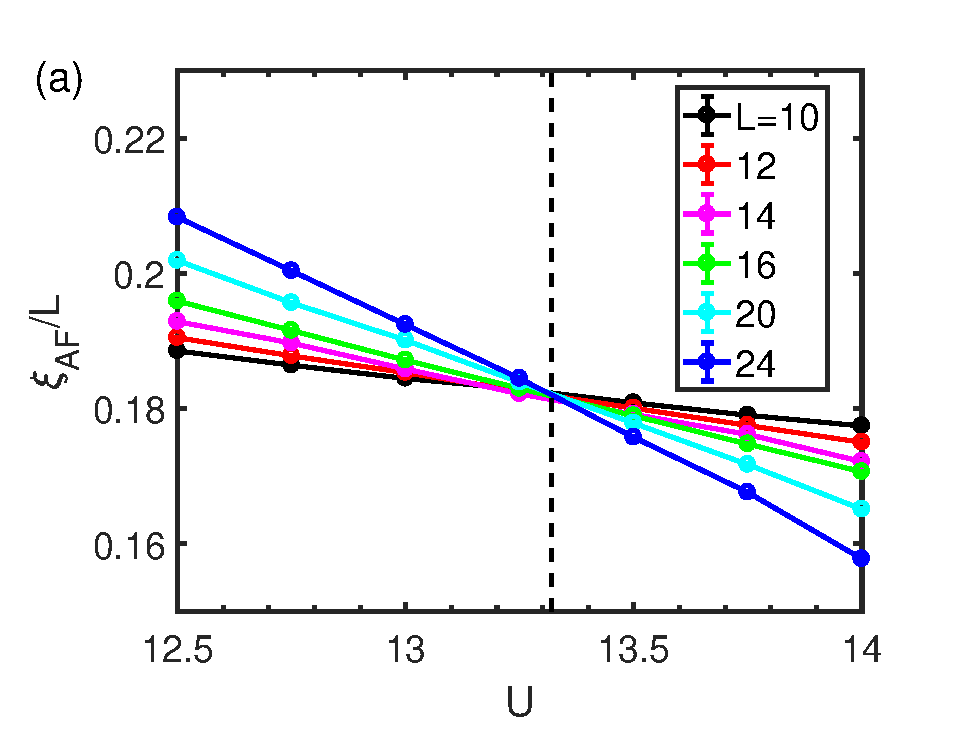
\includegraphics[width=0.45\textwidth]{correlationlength_af}\\
	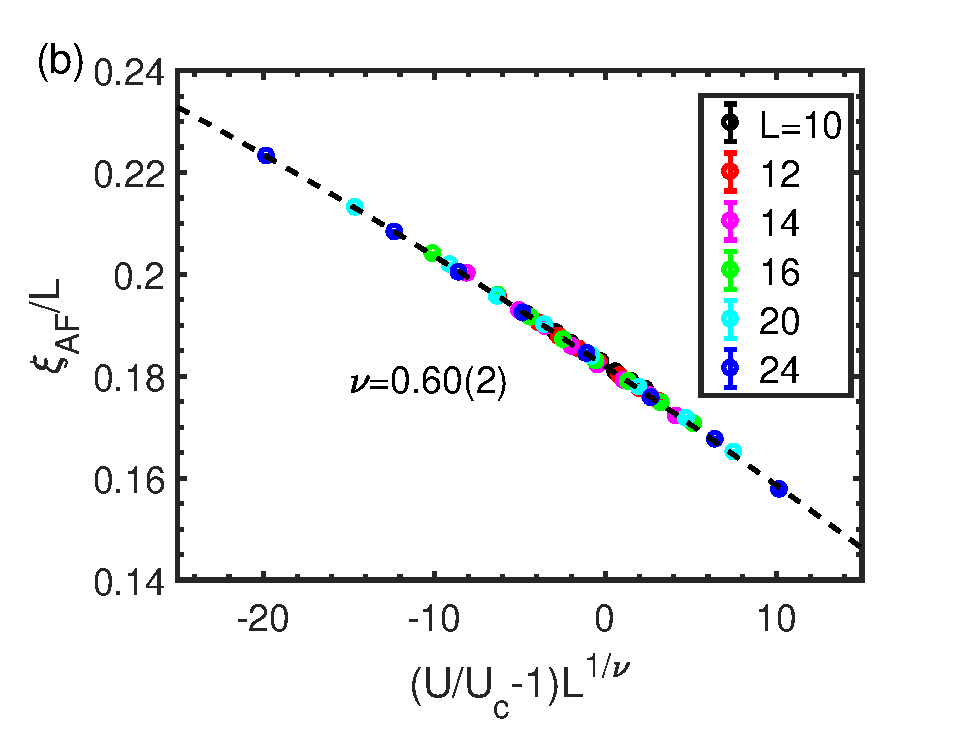
\includegraphics[width=0.45\textwidth]{datacollapse_xi}
	\caption{\label{fig:correlationlength_af} AF correlation length $\xi_{\rm AF}$. (a)$\xi_{\rm AF}/L$ versus $U$ shows a crossing point at $U_c=13.32$. (b)Data collapse of $\xi_{\rm AF}/L$ as a universal function of $(U-U_c)L^{1/\nu}$ with $\nu=0.60(2)$.}
\end{figure}


In parallel to AF, to describe VBS, we define
\begin{eqnarray}
  d_{r\hat{e}}=\sum_{\alpha=1}^{6}\left(c_{r\alpha}^\dag c_{r+\hat{e}\alpha} + c_{r+\hat{e}}^\dag c_{r\alpha} \right)
\end{eqnarray}
where $e=x,y$. The VBS order parameter is then the Fourier transformation at momentum $(\pi,0)$ for $d_x$ and $(0,\pi)$ for $d_y$, i.e. $d_e=\frac{1}{L^2}\sum_r d_{r\hat{e}}(-1)^e$. Again, we omit the momentum index. In QMC simulations, we measure the VBS structure factor 
\begin{eqnarray}
  \langle d^2 \rangle=\frac{1}{L^4}\sum_{rr'} \langle d_{r\hat{e}}d_{r\hat{e}}\rangle (-1)^{r_e-r_e'}
\end{eqnarray}
Here, we have defined the VBS order as a kinetic dimerized order. Such a kinetic definition is not in conflict with the widely used spin-spin definition $d_{r\hat{e}}=\sum_{\alpha\beta}c_{r\alpha}^\dag c_{r\beta} c_{r+\hat{e}\beta}^\dag c_{r+\hat{e}\alpha}$ in spin models, which is just a second order process of the kinetic VBS order.




%\begin{figure}
%  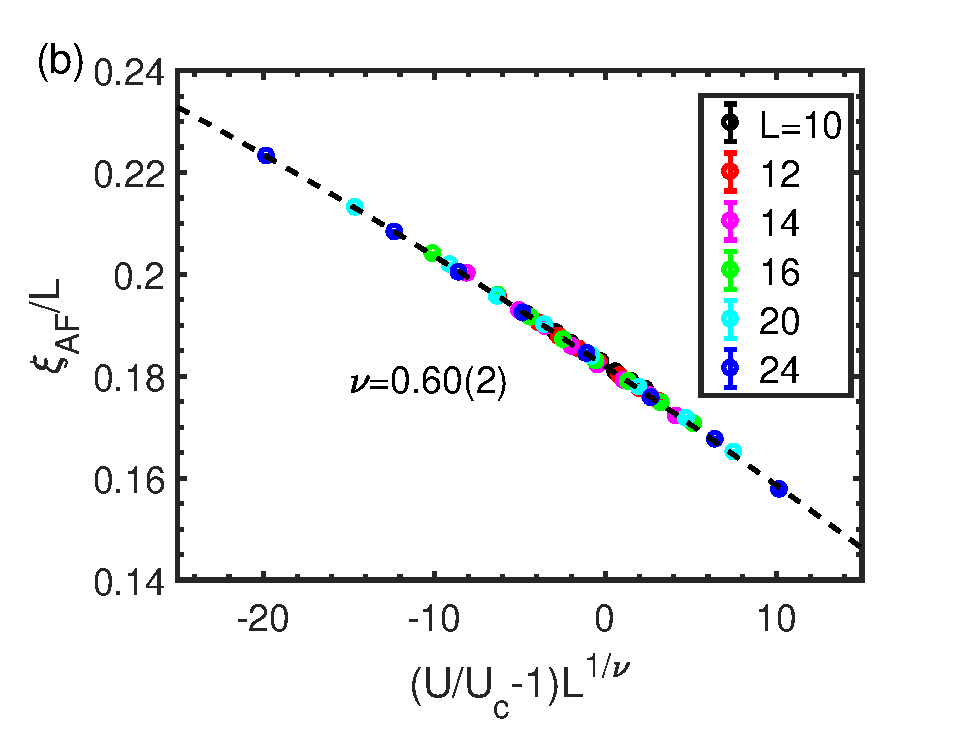
\includegraphics[width=0.45\textwidth]{datacollapse_xi}
%  \caption{\label{fig:datacollapse_xi}Data collapse of $\xi_{\rm AF}$. We plot $\xi_{\rm AF}/L$ as a universal function of $(U-U_c)L^{1/\nu}$ with $\nu=0.60(2)$.}
%\end{figure}
From structure factors, we immediately get the AF correlation length which is defined as \cite{Sandvik2010a}
\begin{eqnarray}
  \xi_{\rm AF}=\frac{1}{q}\sqrt{\frac{\langle m_Q^2 \rangle}{\langle m_{Q+q}^2 \rangle}-1}
\end{eqnarray}
where $Q=(\pi,\pi)$ and $q=(2\pi/L,0)$. When we plot $\xi_{\rm AF}/L$ versus $U$ as shown in Fig.~\ref{fig:correlationlength_af}(a), we find a crossing point at $U_c=13.32(2)$. Furthermore, the $\xi_{\rm AF}$ data are found to collapse to a universal scaling function, as plotted in Fig.~\ref{fig:correlationlength_af}(b), 
\begin{eqnarray}\label{eq:scalinghypothesis}
  \xi_{\rm AF}(U,L)=L f\left[(U-U_c)L^{1/\nu}\right] 
\end{eqnarray}
where the correlation length exponent $\nu$ is determined to be $0.60(2)$. The observation of the universal scaling behavior strongly indicates the phase transition to be a continuous one. 


%The correlation length exponent $\nu$ is defined as $\xi\propto|U-U_c|^{-\nu}$. But since $\xi_{\rm AF}$ and $\xi_{\rm VBS}$ in thermodynamic limit are difficult to obtain, in practice $\nu$ can be determined based on finite size scaling hypothesis \cite{Sandvik2010a}
%\begin{eqnarray}\label{eq:scalinghypothesis}
%A(U,L)=L^\kappa f\left[(U-U_c)L^{1/\nu}\right] 
%\end{eqnarray}
%where $f$ is a universal function and $A$ is a physical quantity which can be $\xi_{\rm AF}$, $\langle m^2 \rangle$ and $\langle d^2 \rangle$ in this work. First, for correlation length $\xi_{\rm AF}$ with $\kappa=1$, we achieve very good data collapse by choosing $\nu=0.60(2)$, as plotted in Fig.~\ref{fig:datacollapse_xi}. 


\begin{figure}
  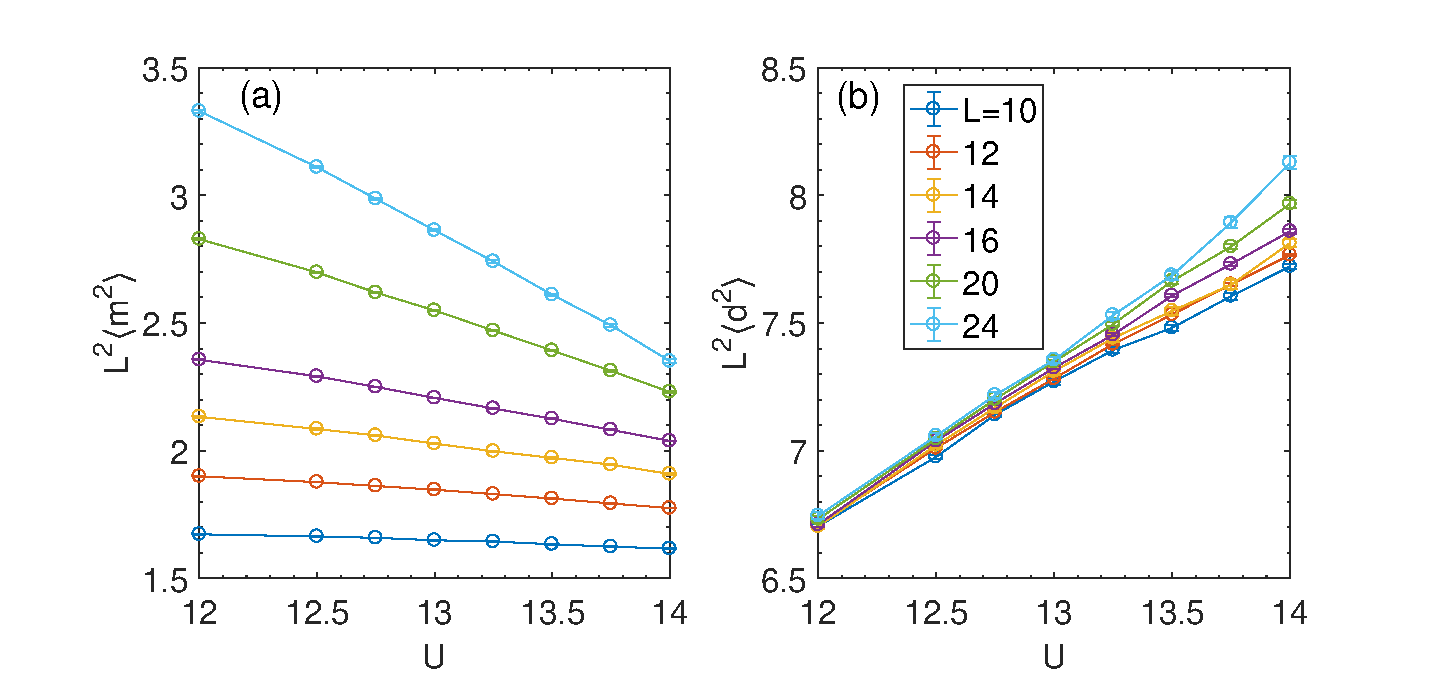
\includegraphics[width=0.53\textwidth]{structurefactor} \\
  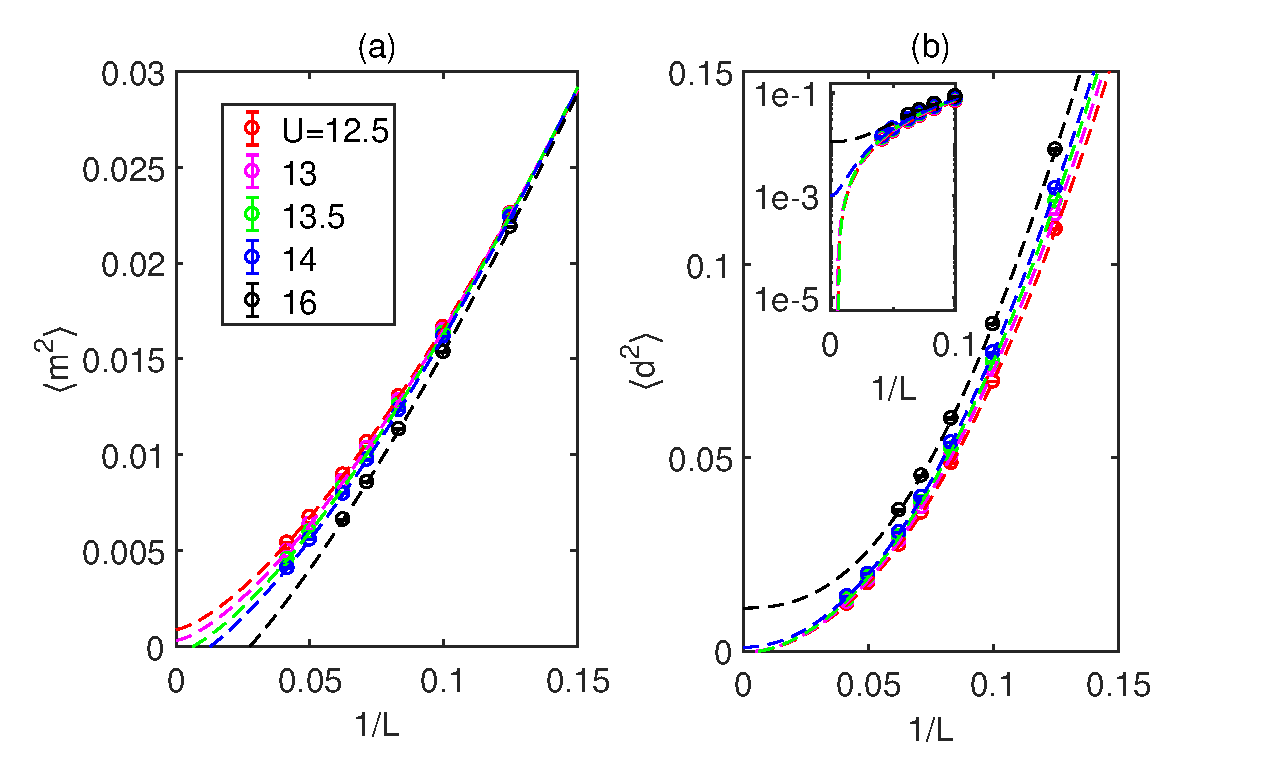
\includegraphics[width=0.53\textwidth]{extrapolation}
  \caption{\label{fig:structurefactor}Structure factors. We plot structure factors of AF and VBS versus $U$ in (a) and (b), respectively. While in (c) and (d), finite size extrapolations versus $1/L$ are performed using Eq.~\ref{eq:extrapolation_magic}.}
  %For AF, no convergence is achieved up to $L=24$, indicating long correlation length $\xi_{\rm AF}$. But for VBS, the structure factor converges as $L$ increases for $U\lesssim13$, indicating much shorter correlation length $\xi_{\rm VBS}$. On the other hand, for $U\gtrsim13.25$, the data of different sizes show clear separation, corresponding to a tendency of long range order.}
\end{figure}
Next, let us check structure factors. Supposing a two-point correlation function $\langle m_rm_0 \rangle=(-1)^r(M^2 + \delta\mathrm{e}^{-r/\xi})$ as $r\rightarrow\infty$ which is always true as long as we are away from the critical point, we obtain the structure factor after a Fourier transformation 
\begin{eqnarray}\label{eq:extrapolation}
  \langle m^2 \rangle=M^2+a\frac{\xi^2}{L^2}
\end{eqnarray}
as long as $L\gg\xi$. As a result, as $L$ increases $L^2\langle m^2 \rangle$ saturates to a fixed value $a\xi^2$ in disordering phase while diverges in the ordering phase. From the raw data of AF and VBS structure factors as functions of $U$ shown in Fig.~\ref{fig:structurefactor}(a,b), we get the information that $\xi_{\rm AF}\gg\xi_{\rm VBS}$. The VBS curves begin to separate around $U\approx13.25$ indicating the onset of the VBS long range order, while the AF data show almost no significant change because of the large $\xi_{\rm AF}$. Therefore, we resort to finite size extrapolation to extract their thermodynamic values. 


%\begin{figure}
%  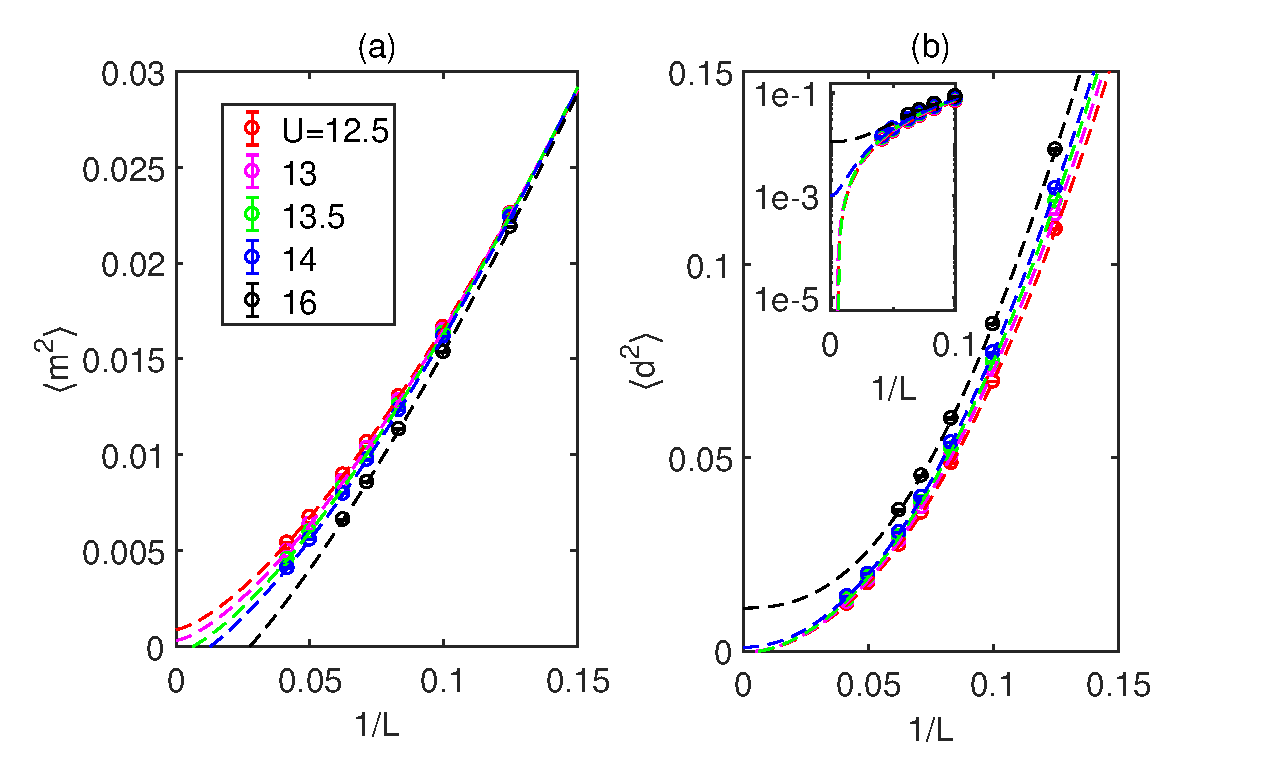
\includegraphics[width=0.53\textwidth]{extrapolation}
%  \caption{\label{fig:extrapolation}Finite size scalings. We plot fittings of $\langle m^2 \rangle$ (a) and $\langle d^2 \rangle$ (b) as functions of $1/L$ . The power law polynominal with a subleading correction $y(x)=y_0+a/(L^2+bL^\omega)$  is used to fit the QMC data.}
%\end{figure}

\begin{figure}
  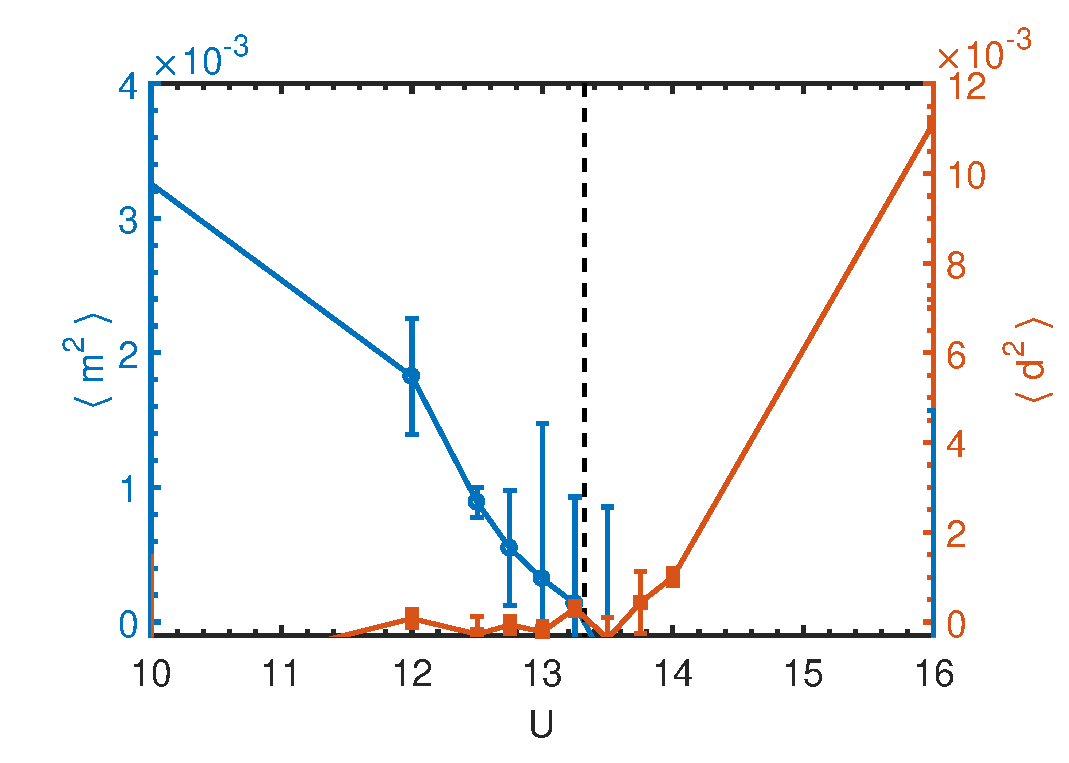
\includegraphics[width=0.4\textwidth]{phasediagram}
  \caption{\label{fig:phasediagram}Phase diagram. The extrapolation values of $\langle m^2 \rangle$ and $\langle d^2 \rangle$ are plotted together. The error bars are determined by the $95\%$ confidence bounds of the finite size data fittings. The large error bars near the critical point mainly come from our extrapolation method which contains four fitting parameters but the number of data points is limited by lattice size $L\le24$. The dashed line indicates the phase transition point $U_c=13.32$ which is obtained from the data crossing of $\xi_{\rm AF}/L$ vs $U$ as shown in Fig.~\ref{fig:correlationlength_af}(a).}
\end{figure}

Generally speaking, finite size extrapolation is not an easy task, especially when the system size $L$ is not large enough. However, in our case, we have found Eq.~\ref{eq:extrapolation} together with a subleading correction \cite{Sandvik2010a} i.e.
\begin{eqnarray}\label{eq:extrapolation_magic}
  \langle m^2 \rangle=M^2+\frac{a}{L^2+bL^\omega}
\end{eqnarray}
works astonishingly well. Here, $M^2$, $a$, $b$ and $\omega$ are fitting parameters determined by a standard non-linear least square method. 
%The weight $w_i$ of a given data $x_i$ is determined by its QMC error bar $w=1/\Delta x_i^2$. 
In Fig.~\ref{fig:structurefactor}(c,d) we plot several representative fitting results with data of $L\ge8$. From the extrapolation values, we find $\langle m^2 \rangle$ decreases and finally vanishes as $U$ increases while $\langle d^2\rangle$ shows the opposite behavior. We collect all extrapolation values and put them together to obtain the phase diagram as shown in Fig.~\ref{fig:phasediagram}. From the phase diagram, we see a clear AF-VBS phase transition which seems like a continuous or weakly first order one.






Another signature of the continuous phase transition comes from the energy per site $E$ versus $U$ as shown in Fig.~\ref{fig:energydoublon}(a) and also double occupation $\langle n_\alpha n_\beta \rangle$ ($\alpha\ne\beta$) which corresponds to the energy derivative $\partial E/\partial U$ in Fig.~\ref{fig:energydoublon}(b). Both $E$ and its derivative show convergence with size $L$ without any singularity strongly confirming the continuous phase transition. From the large value of double occupation, we recognize that $U$ in our simulations is not large enough such that charge fluctuation is not totally forbidden but is quite strong. This is a fundamental difference between our fermionic model and extensively studied spin models in literature.

\begin{figure}
	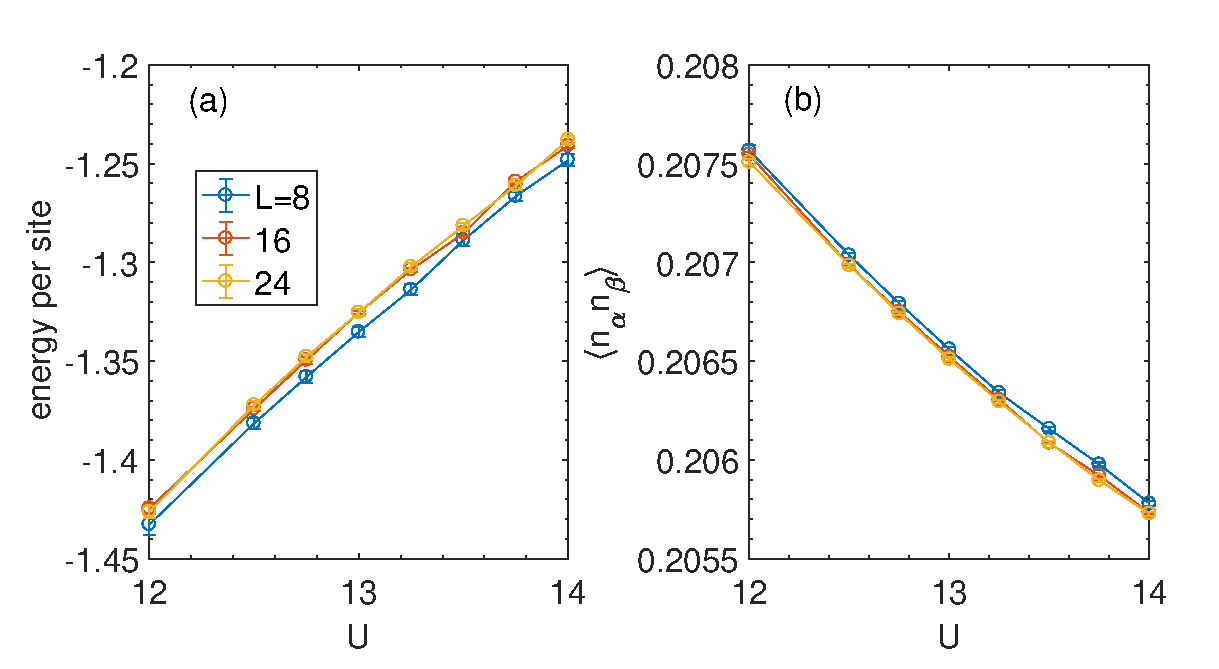
\includegraphics[width=0.5\textwidth]{energydoublon}
	\caption{\label{fig:energydoublon}Energy and double occupation. In (a), we plot energy per site $E$ versus $U$ for $L=8$, $16$ and $24$, respectively. The data show a convergence without any singularity. In (b), we also plot double occupation $\langle n_\alpha n_\beta \rangle$, which gives the energy derivative $\partial E/\partial U$ and shows no singularity as well.}
\end{figure}

\begin{figure}
  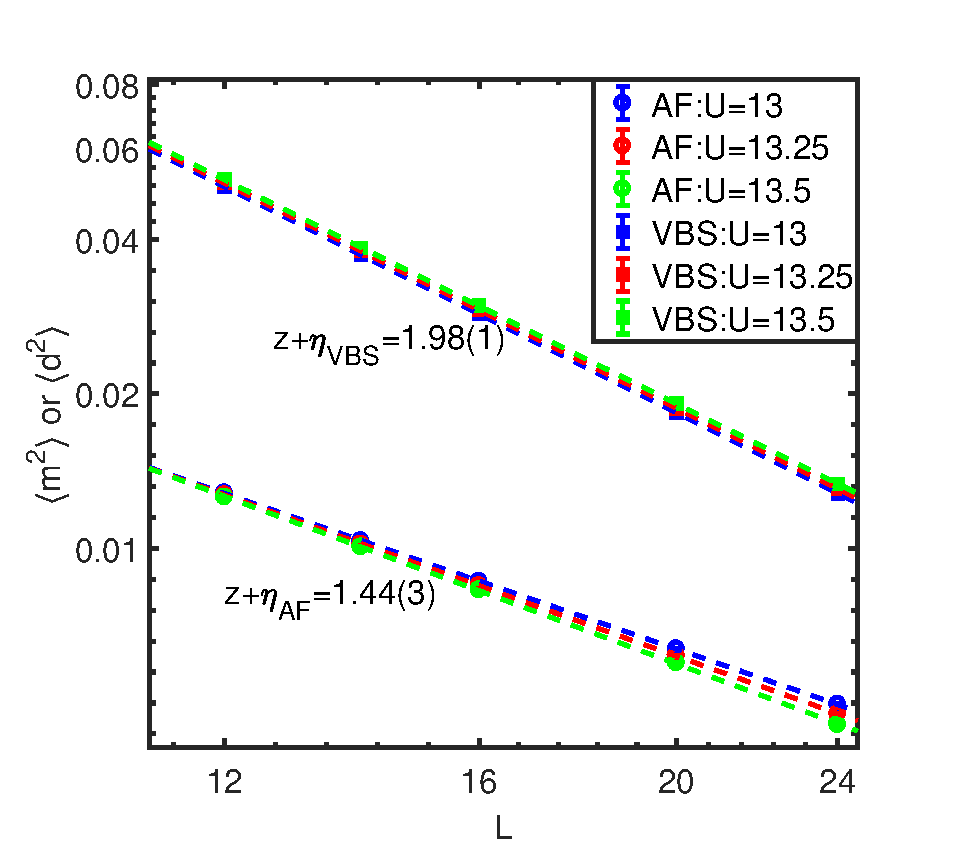
\includegraphics[width=0.5\textwidth]{etaexponent}
  \caption{\label{fig:etaexponent}Anomalous dimensions. We plot structure factors $\langle m^2 \rangle$ and $\langle d^2 \rangle$ versus $L$ near the critical point, respectively, using log-log plots. Dashed lines are linear fittings. From their slopes we obtain anomalous dimensions $\eta_{\rm AF}=0.44(3)$ and $\eta_{\rm VBS}=0.98(1)$ after taking the dynamical exponent $z=1$. }
\end{figure}

%\begin{figure}
%  \includegraphics[width=0.53\textwidth]{datacrossing}
%  \caption{\label{fig:datacrossing}Data crossing of structure factors. We plot $L^{z+\eta_{\rm AF}}\langle m^2 \rangle$ and $L^{z+\eta_{\rm VBS}}\langle d^2 \rangle$ versus $U$ in (a) and (b), respectively. Both plots show a data crossing at the phase transition point indicated by the dashed lines. For VBS, the data crossing is not so clear with our QMC data, due to the large value of $\eta_{\rm VBS}$ and short correlation length $\xi_{\rm VBS}$ which require higher data quality to pin down the transition point more accurately.}
%\end{figure}

At the critical point, two-point correlation function in 2+1 dimension is expected to be algebraic decay as $\langle m_rm_0\rangle\sim r^{-z-\eta}$. \cite{Sondhi1997} After a Fourier transformation, we find the structure factor satisfies the same power law
\begin{eqnarray}
  \langle m^2 \rangle \sim \frac{1}{L^{z+\eta}}
\end{eqnarray}
as long as $L$ is large enough.
In Fig.~\ref{fig:etaexponent} we plot $\langle m^2 \rangle$ and $\langle d^2\rangle$ versus $L$ on a log-log coordinate around $U_c=13.32(2)$. Up to the maximal available lattice size $L=24$, we find good linear fittings. From the slopes, we obtain the anomalous dimension $\eta_{\rm AF}=0.44(3)$ and $\eta_{\rm VBS}=0.98(1)$ after taking the dynamical exponent $z=1$ according to both theories and other numerical works on deconfined QCP. \cite{Senthil2004,*Senthil2004a,*Levin2004,Sandvik2007} 
%The values of the two anomalous dimensions are further confirmed by data crossings when we plot $L^{z+\eta_{\rm AF}}\langle m^2 \rangle$ and $L^{z+\eta_{\rm VBS}}\langle d^2 \rangle$ versus $U$, as shown in Fig.~\ref{fig:datacrossing}. 
In our model, the large values of $\eta_{\rm AF}$ and $\eta_{\rm VBS}$ can be taken as an evidence of the deconfined QCP because the existence of deconfined spinons strongly quickens the decay of two-point correlation functions. Moreover, the values of $\eta_{\rm AF}$ and $\eta_{\rm VBS}$ here are different from those of the fundamental representation case corresponding to CP$^{5}$ model (where $\eta_{\rm AF}\approx0.56$ and $\eta_{\rm VBS}\approx1.15$), \cite{Kaul2012a} indicating they belong to different universality classes.
Next, when we tried to plot $L^{z+\eta_{\rm AF}}\langle m^2 \rangle$ and $L^{z+\eta_{\rm VBS}}\langle d^2 \rangle$ versus $(U-U_c)L^{1/\nu}$, we failed to obtain good data collapses (not shown here). Of course, this may be caused by small lattice size in our QMC simulations. But another more physically relevant reason may be the recently proposed two-length scaling hypothesis \cite{Senthil2004,Shao2016} while our QMC simulations with small size up to $L=24$ prevent us to perform such an ingenious scaling analysis.



%\begin{figure}
%  \includegraphics[width=0.45\textwidth]{../datacollapse_af}
%  \caption{\label{fig:datacollapse_af}Data collapse of AF structure factor. By tuning $\nu_{\rm AF}=0.44(3)$, we achieve a data collapse of $L^{z+\eta_{\rm AF}}\langle m^2 \rangle$ as a universal function of $(U-U_c)L^{1/\nu_{\rm AF}}$ regardless of $L$. }
%\end{figure}



%Next, let us examine the scaling behavior of AF and VBS structure factors. For AF, we can achieve data collapse by choosing another exponent $\nu_m=0.44(3)$ different from the above $\nu=0.60(2)$, as shown in Fig.~\ref{fig:datacollapse_af}. This discrepancy can not be explained in the single parameter scaling hypothesis Eq.~\ref{eq:scalinghypothesis} but is not in conflict with the recently proposed many parameter hypothesis in which more than one divergent correlation length give more than one exponent $\nu$. \cite{Shao2016} The failure of Eq.~\ref{eq:scalinghypothesis} is further seen in Fig.~\ref{fig:datacollapse_vbs} for the VBS structure factor, where we have to choose a much larger $\nu_d$, say $1<\nu_d<4$ or $\nu_d\approx2.5$. 


%\begin{figure}
%  \includegraphics[width=0.5\textwidth]{../datacollapse_vbs}
%  \caption{\label{fig:datacollapse_vbs}Data collapse of VBS structure factor. We try to find out the best value of correlation length exponent $\nu_d$ by data collapse of $L^{z+\eta_{\rm VBS}}\langle d^2 \rangle$. By setting $\nu_d=\nu_m$ as shown in (a), we failed to get a data collapse. (b), (c) and (d) show plots with $\nu_d=1$, $2.5$, and $4$, respectively. From the results, we conclude $\nu_d$ is very large, at least larger than $1$. }
%\end{figure}

%\subsection{emergent U(1) symmetry of VBS}


\begin{figure}
  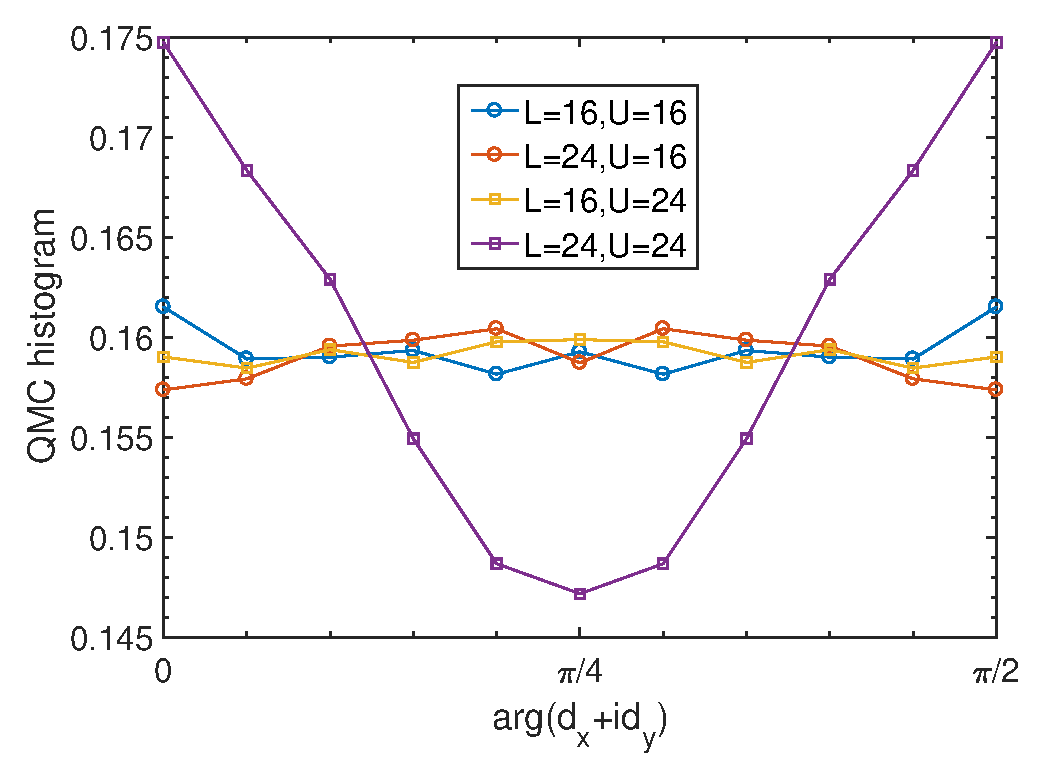
\includegraphics[width=0.4\textwidth]{histogram_vbs}
  \caption{\label{fig:histogram_vbs}QMC histogram of the argument of VBS order parameter $(d_x+id_y)$. }
\end{figure}

According to deconfined quantum criticality, the VBS order parameter changes its symmetry from $Z_4$ to U(1) as approaching the QCP. \cite{Senthil2004,*Senthil2004a,*Levin2004} In order to check this emergent U(1) symmetry, we measured the histogram of VBS configurations during QMC samplings. \cite{Sandvik2007} For each QMC configuration, we obtain a data point $(d_x,d_y)$. Plotting the histogram of $\mathrm{arg}(d_x+id_y)$, we obtain Fig.~\ref{fig:histogram_vbs}. For $U=24$ and $L=24$ which is deep inside the VBS phase, a significant $Z_4$ feature is observed corresponding to the columnar VBS. When we go approaching the critical point by reducing $U$ or $L$, the $Z_4$ feature becomes weaker as a result of stronger fluctuations, in consistent with an emergent U(1) symmetry at the deconfined QCP. 



\section{summary}

In summary, based on QMC simulations, we have found the signatures of the deconfined QCP at $U_c=13.32(2)$ in the half-filled SU(6) Hubbard model on a square lattice. By symmetry analysis, the observed QCP belongs to a universality class called $U(N)/[U(N/2)\otimes U(N/2)]$ model which is different from the CP$^{N-1}$ model. The fully understanding, e.g. critical exponents, of the self-conjugate (or multi-rows in general) represented theory beyond the CP$^{N-1}$ model calls for more theoretical efforts, e.g. $1/N$ expansion or renormalization group analysis in the future.

\section{acknowledgement}
We thank xxx.
We are supported by grant yyy.
Our numerical calculations are performed on Tianhe-II. 

\bibliography{all}
\end{document}
